\section{Synchronizing the ratios and arranging the scales}
\label{sec:synchronization}

The normalized problem is the following. It is the only part of the
geometric theorem requiring control of uncountably many ratios at once.

\begin{proposition}[Uniform normalized hitting]\label{prop:normalized}
Let $0<\alpha<\beta<1$ and $0<p<1$. There is an open $1$-periodic
set $H\subset\R$ such that $\rho(H)\le6p$ and
\begin{equation}\label{eq:normalized-hit}
 \forall x\in\R\ \forall t\in[1,2]\ \forall q\in[\alpha,\beta]
 \quad \exists n\ge1:\ x+tq^n\in H.
\end{equation}
\end{proposition}

The parameters $\alpha,\beta,p$ are fixed until \cref{sec:global}.
Choose $Q$ and an integer $T\ge1$ with
\begin{equation}\label{eq:Q-T}
 0<Q<\frac\alpha2,\qquad \beta^T\le Q,
 \qquad c=\frac4{\alpha-Q}.
\end{equation}
These choices can be rational when the input parameters are rational.

\subsection{A subsequence at prescribed logarithmic scales}

For $j\ge1$ and $q\in[\alpha,\beta]$, define
\begin{equation}\label{eq:nu}
 \nu_j(q)=\min\{n\ge1:q^n\le Q^j\},
 \qquad a_j(q)=q^{\nu_j(q)}.
\end{equation}
Thus $a_j(q)$ is a term of the original progression, selected just as it
passes the level $Q^j$. Only the selection of test points depends on $q$;
the grids, random tables, and final hitting set will not.

\begin{lemma}[Uniform envelopes and separation]\label{lem:envelopes}
For every $j\ge1$ and $q\in[\alpha,\beta]$,
\begin{equation}\label{eq:envelope}
 \alpha Q^j<a_j(q)\le Q^j,\qquad \nu_j(q)\le Tj.
\end{equation}
The integers $\nu_j(q)$ strictly increase in $j$. If $j<j'$, then
\begin{equation}\label{eq:sample-gap}
 a_j(q)-a_{j'}(q)>(\alpha-Q)Q^j.
\end{equation}
For fixed $j$, $\nu_j(q)$ is a nondecreasing integer step function of $q$,
with at most $Tj$ possible jump locations on $[\alpha,\beta]$.
\end{lemma}

\begin{proof}
Minimality gives $q^{\nu_j(q)-1}>Q^j$, including when the preceding
exponent is zero. Multiplication by $q\ge\alpha$ proves the strict
lower bound in \eqref{eq:envelope}; its upper bound is the definition.
Also $q^{Tj}\le\beta^{Tj}\le Q^j$, so $\nu_j(q)\le Tj$.
For $j'>j$, $a_{j'}(q)\le Q^{j'}\le Q^{j+1}$, whereas
$a_j(q)>\alpha Q^j$. Subtraction proves \eqref{eq:sample-gap}, and in
particular the selected original indices are distinct.
Finally the condition $\nu_j(q)\le n$ is equivalent to $q^n\le Q^j$.
Changes can occur only at $q=Q^{j/n}$ for integers $1\le n\le Tj$.
At equality the minimum in \eqref{eq:nu} specifies the value; no
continuity at a jump is assumed.
\end{proof}

\begin{remark}
Directly using a grid adapted to $\alpha^j$ for all $q\in[\alpha,\beta]$
would compare later displacements of size $\beta^a$ with earlier cells
of size $\alpha^b$. The factor $(\beta/\alpha)^b$ then destroys uniform
stability. The selected terms in \eqref{eq:nu} replace this comparison
by $Q^{a-b}$, independent of the ratio.
\end{remark}

\begin{figure}[htbp]
\centering
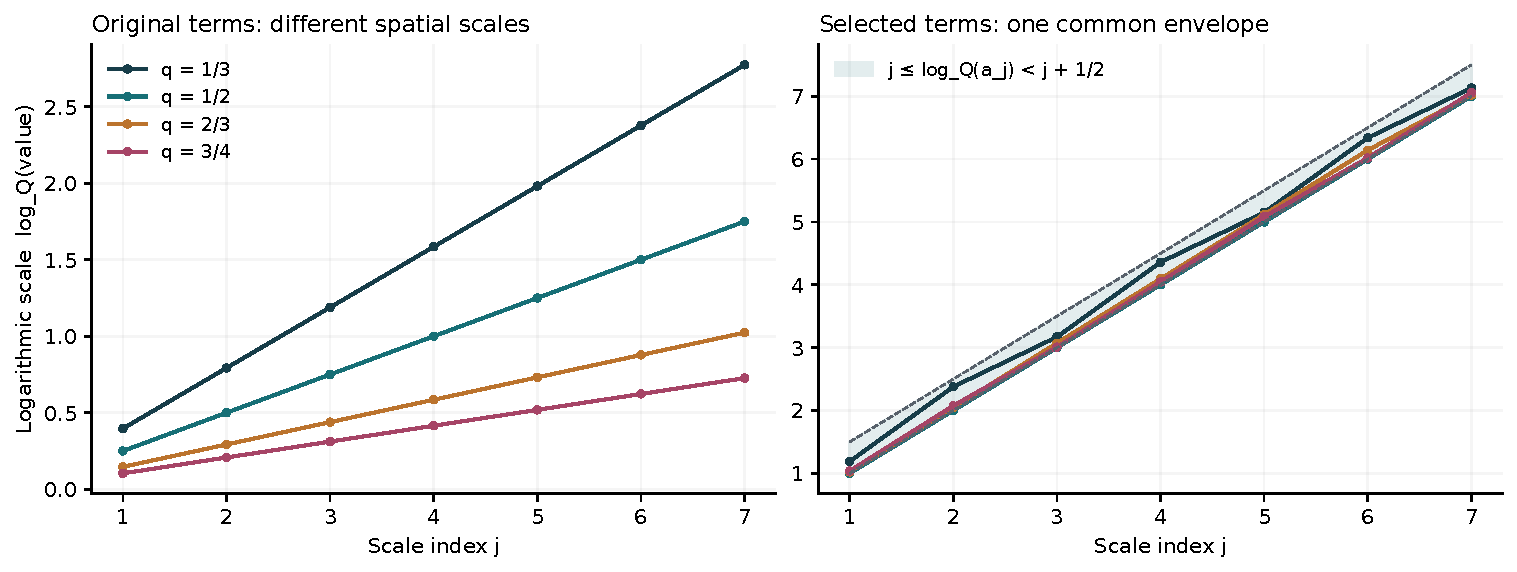
\includegraphics[width=\textwidth]{figures/synchronized_scales.pdf}
\caption{An exact sampling rule brings different ratios onto common scales.
The displayed example uses $Q=1/16$, $\alpha=1/4$, and four rational ratios.
On the right, the selected values satisfy
$j\le\log_Q a_j<j+1/2$, so the same spatial resolutions work for every
curve. The plot illustrates \cref{lem:envelopes}; the proof does not rely
on the finite set of ratios shown.}
\label{fig:sync}
\end{figure}

\subsection{One nested family of grids}

For integers $b\ge1$ choose
\begin{equation}\label{eq:grids}
 N_b=2^{\lceil\log_2(cQ^{-b})\rceil},\qquad
 \Gamma_b=N_b^{-1}\Z,\qquad
 J_b(z)=\lfloor N_b\{z\}\rfloor.
\end{equation}
Here $\{z\}$ is the fractional part. The cells are closed on the left
and open on the right, and
\begin{equation}\label{eq:grid-size}
 cQ^{-b}\le N_b<2cQ^{-b}.
\end{equation}
Since the $N_b$ are nondecreasing powers of two, every finer key determines
all coarser keys. This fact concerns actual periodic cells, including
cells adjacent to an integer.

\subsection{Preorder windows and their exact span}

Fix integers $M\ge2$, $d\ge1$, $g\ge1$, and $r_0\ge1$, to be chosen
in that order later. Let $\mathcal T$ be a complete ordered $M$-ary tree
of height $d$. Leaves have height zero. Write $P_i$ for the $i$th child
of $P$. An edge $e=(P,i)$ is listed immediately before all edges below
$P_i$, and that whole block precedes $(P,i+1)$. This is preorder.
Let
\begin{equation}\label{eq:Kedges}
 K=M+M^2+\cdots+M^d
\end{equation}
be the number of edges.

Each edge receives an integer window $W_e=[a_e,b_e]\cap\Z$.
Place the windows in preorder, with exactly $g$ unused indices between
successive windows. All edges from a height-$h$ vertex receive length
$r_h$. Define the subtree spans by
\begin{align}
 r_1&=r_0,& \sigma_1&=Mr_0+(M-1)g,\label{eq:window-recursion1}\\
 r_h&=g+\sigma_{h-1},&
 \sigma_h&=2M\sigma_{h-1}+(3M-1)g\quad(2\le h\le d).
 \label{eq:window-recursion2}
\end{align}
Every $r_h\ge r_0$. The expression for $\sigma_h$ counts $M$ blocks
consisting of an outgoing window, one gap, and its child subtree, together
with $M-1$ gaps between those blocks.

Start the first window at a fixed $j_0\ge1$ with $2Q^{j_0}\le1/4$.
Let
\begin{equation}\label{eq:B-global}
 B=j_0-1+\sigma_d,\qquad \mathcal J=\bigcup_e W_e.
\end{equation}
The letter $B$ always denotes this largest window index; the random set
will be denoted $A$.

For an edge $e$, let $b_e^*$ be the largest index in its own window or
any window in its child subtree.

\begin{lemma}[Local span and global affine growth]\label{lem:span}
If $e$ leaves a height-$h$ vertex, then
\begin{equation}\label{eq:span}
 b_e^*-a_e+1\le2r_h.
\end{equation}
For fixed $M,d,g,j_0$, the value $B$ is an affine function of $r_0$.
Explicitly,
\begin{align}
 \sigma_d={}&M(2M)^{d-1}r_0\notag\\
 &+\left((M-1)(2M)^{d-1}
 +(3M-1)\frac{(2M)^{d-1}-1}{2M-1}\right)g.
 \label{eq:affine-span}
\end{align}
\end{lemma}

\begin{proof}
For a leaf edge the span equals $r_1$. Otherwise preorder makes the
edge--subtree span exactly $r_h+g+\sigma_{h-1}=2r_h$.
Solving the affine recurrence \eqref{eq:window-recursion2}, starting
from \eqref{eq:window-recursion1}, gives \eqref{eq:affine-span}.
\end{proof}

The local bound \eqref{eq:span} controls the parameter count. The
separate global bound \eqref{eq:affine-span} ensures that polynomial
losses in $B$ can be absorbed by increasing $r_0$. Replacing every
local resolution by the finest grid of the entire tree would lose
this separation of roles.

\subsection{Stable centers and distinct addresses}

Call $x\in\R$ \emph{stable} if for every window except the first,
with $b'$ the endpoint of its immediate predecessor,
\begin{equation}\label{eq:stable-def}
 (x,x+2Q^{a_e}]\cap\Gamma_{b'}=\varnothing.
\end{equation}
Let $\calS$ be the stable set.

\begin{lemma}[Uniform stability]\label{lem:stable}
The set $\calS$ is measurable and $1$-periodic, and
\begin{equation}\label{eq:unstable-density}
 \rho(\R\setminus\calS)\le4KcQ^{g+1}.
\end{equation}
If $x\in\calS$, $j\in W_e$, $t\in[1,2]$, and
$q\in[\alpha,\beta]$, then every edge $f$ preceding $e$ satisfies
\begin{equation}\label{eq:earlier-key}
 J_{b_f}(x+ta_j(q))=J_{b_f}(x).
\end{equation}
\end{lemma}

\begin{proof}
The centers violating one condition in \eqref{eq:stable-def} lie in
$\bigcup_{\gamma\in\Gamma_{b'}}[\gamma-2Q^{a_e},\gamma)$.
Its density is at most $2N_{b'}Q^{a_e}<4cQ^{a_e-b'}=4cQ^{g+1}$.
A union bound over fewer than $K$ conditions proves
\eqref{eq:unstable-density}. For a stable center, the displacement
$ta_j(q)$ belongs to $(0,2Q^{a_e}]$, so it crosses no boundary of the
predecessor grid. A boundary at $x$ itself belongs to its right-hand
cell and causes no exception. Nestedness gives the assertion at every
earlier resolution.
\end{proof}

\begin{lemma}[Separation within a window]\label{lem:separation}
For every edge $e$ and every fixed $(x,t,q)$ in the stated ranges, the
points
\[
 \{x\}\cup\{x+ta_j(q):j\in W_e\}
\]
have pairwise distinct keys at resolution $b_e$ and at all finer
resolutions.
\end{lemma}

\begin{proof}
All points lie in an interval of length at most $2Q^{j_0}\le1/4$;
their ordinary distances therefore equal their circular distances.
Their distances from the center are greater than $\alpha Q^{b_e}$.
By \eqref{eq:sample-gap}, the distance between two translated points
is greater than $(\alpha-Q)Q^{b_e}$. But a cell has width at most
$Q^{b_e}/c=(\alpha-Q)Q^{b_e}/4$. Two points sharing a key have circular
distance less than that width. Thus the keys are distinct, and remain
so at finer resolutions.
\end{proof}
